\documentclass[11pt]{article}
%% Set my margins
\setlength{\oddsidemargin}{0.0truein}
\setlength{\evensidemargin}{0.0truein}
\setlength{\textwidth}{6.5truein}
\setlength{\topmargin}{0.0truein}
\setlength{\textheight}{9.0truein}
\setlength{\headsep}{0.0truein}
\setlength{\headheight}{0.0truein}
\setlength{\topskip}{0pt}
%% End of margins

\usepackage[pdftex,
bookmarks,
bookmarksopen,
pdfauthor={Jin Liu},
pdftitle={REMI Vignette}]
{hyperref}

\title{`\texttt{REMI}' Package to conduct regression with marginal information with applications in genome-wide association studies}
\author{Jian Huang$~^1$, Yuling Jiao$~^{2}$, Jin Liu$~^3$, and Can Yang$~^4$\\
$~^1$ Department of Applied Mathematics, Hong Kong Polytechnics
University, Hong Kong.\\
$~^2$ Department of Statistics, Zhongnan University of Economics and Law, China.\\
$~^3$ Centre for Quantitative Medicine, Duke-NUS Graduate Medical School, Singapore.\\
$~^4$ Department of Mathematics, The Hong Kong University of Science and Technology,\\
Hong Kong.\\
}

\date{\today}



\usepackage{Sweave}
\begin{document}
\input{REMI_packages-concordance}
\maketitle

\section{Overview}
This vignette provides an introduction to the `\texttt{REMI}' package.
R package `\texttt{REMI}' implements REMI, an efficient statistical approach to conduct \underline{RE}gression with \underline{M}arginal \underline{I}nformation with an application in genome-wide association studies (GWAS).

The package can be installed with the command:
%<<REMI-prelim, warning=FALSE>>=
%#install.packages("devtools")
%library(devtools)
%install_github("gordonliu810822/REMI")
%@
\begin{verbatim}
> #install.packages("devtools")
> library(devtools)
> install_github("gordonliu810822/REMI")
\end{verbatim}

The package can be loaded with the command:
%<<REMI-prelim, warning=FALSE>>=
%library("REMI")
%@
\begin{verbatim}
> library("REMI")
\end{verbatim}

This vignette is organized as follows.
Section~\ref{datagene} shows how we use the real genotype data to generate phenotype data.
Section~\ref{REMIfit} shows how we fit two versions of REMI (REMI-C and REMI-R). If you have any problems running the demo, please contact Jin Liu at \texttt{jin.liu@duke.nus.edu.sg}. Before running this demo, please download all the demo data sets at \url{https://drive.google.com/drive/folders/1ic9Q7Onq0iDNSkex-S4V_YRv-_aL4UxL?usp=sharing}.

\section{Data}
\label{datagene}
In this vignette, we use the 3,200 individuals's real genotype data from GERA in chromosome 16 to chromosome 18 (19,865 SNPs) to generate a phenotype. First, we use an function embeded within `\texttt{REMI}' package to read data from PLINK bed, bim, fam files directly as
\begin{verbatim}
> n1 = 3000;
> dat = ReadPlinkFile('eur_chr16.17.18_3000');
> x = dat$X;
\end{verbatim}
We use 3,000 of all samples as training set and rest 200 samples as testing set by
\begin{verbatim}
> keeplist = read.table(paste("keeplist_",n1,sep=""),sep="\t",header=F)
> fam = read.table(paste("eur_chr16.17.18_",n1,".fam",sep=""),sep=" ",header=F)
> test.set = match(keeplist[1:200,1],fam[,1]);
> train.set = match(keeplist[201:dim(x)[1],1],fam[,1]);
> train.lasso.set = match(keeplist[201:3200,1],fam[,1]);
\end{verbatim}
To conduct REMI, we need a reference panel to estimate the correlation or covariance structure among covariates. Here, we use 1000 Genome Project (1000G) data as reference panel data. Thus, we need match reference allele in GERA with 1000G for each SNP. Here we load reference allele information from GERA first as
\begin{verbatim}
> frq = read.table('eur_chr16.17.18_3000.frq',header=T);
> rsname = as.character(unlist(frq[,2]))
> A1_raw = as.character(unlist(frq[,3]))
\end{verbatim}

The phenotype data is generated using linear model and 0.1$\%$ of SNPs have non-zero effects following Gaussian distribution. We simulate the phenotype data such that the heritability is controlled at 0.5. The codes are
\begin{verbatim}
> p = dim(x)[2]; #n =dim(x)[1];
> alpha= 0.005;
> m = as.integer(alpha*p);
> h2 = 0.5;
> eps = 0.2;
> set.seed(10000)
> b = numeric(p);
> indx = sample(1:p,m);
> b[indx] = rnorm(m);
> n = dim(x)[1]
> y0 = x%*%b;
> y = y0 + rnorm(n)*sd(y0)*sqrt((1-h2)/h2);
> var(y0)/var(y)
>
> ytrain.lasso = y[train.lasso.set];
> xtrain.lasso = x[train.lasso.set,];
> ytrain = y[train.set];
> xtrain = x[train.set,];
> ytest = y[test.set];
> xtest = x[test.set,];
>
> x_var = apply(xtrain.lasso*xtrain.lasso,2,sum);
> yc.lasso = ytrain.lasso - mean(ytrain.lasso);
> Xmean.lasso = apply(xtrain.lasso, 2, mean);
> xc.lasso= sweep(xtrain.lasso,2,Xmean.lasso)
\end{verbatim}

Then, summary statistics can be generated as
\begin{verbatim}
> Xmean = apply(xtrain, 2, mean);
> xc= sweep(xtrain,2,Xmean);
> yc = ytrain - mean(ytrain);
> ytilde = numeric(p);
> betah = numeric(p); s2 = numeric(p);
> for (i in 1:p){
  fm = lm(yc~1+xtrain[,i]);
  betah[i] = summary(fm)$coefficients[2,1];
  s2[i] = summary(fm)$coefficients[2,2]^2;
  ytilde[i] = sum(yc*xc[,i])/length(yc);
}
\end{verbatim}

Then, the files with summary statistics are created as

\begin{verbatim}
# rs, A1, A2, betah, se2, n
# summary statistics for REMI-R
> sumdat = data.frame(rsname,frq[,3:4],betah, s2, rep(n,p))
> write.table(sumdat, "sumdat_sim1.txt",sep=" ",quote=F, row.names=F,col.names=F)
# summary statistics for REMI-C
> sumdat2 = data.frame(rsname[1:p],frq[1:p,3:4],ytilde, rep(var(y),p), rep(n,p))
> write.table(sumdat2, "sumdat_sim2.txt",sep=" ",quote=F, row.names=F,col.names=F)
\end{verbatim}

\section{Fit REMI}
\label{REMIfit}
The REMI-R and REMI-C are fitted as
\begin{verbatim}
> plink_file = "all_chr_1000G_sim_chr16.17.18";
> summarystat_file1 = "sumdat_sim1.txt"
> summarystat_file2 = "sumdat_sim2.txt"
> out = REMI_R(summarystat_file1, plink_file,epsilon=0.2)
> out2= REMI_C(summarystat_file2, plink_file,epsilon=0.2);
\end{verbatim}
where \texttt{plink$\_$file} is 1000G reference penale data.

\section{Plot Solution Paths}
Fit Lasso using genotype data first by
\begin{verbatim}
> sp= lasso(xtrain.lasso,yc.lasso,x_var,100,eps)
\end{verbatim}
The solution path for Lasso, REMI-R and REMI-C are produced by
\begin{verbatim}
> png(filename = "path_demo.png", width = 360, height = 120, units = "mm",res=600)
> par(mfrow=c(1,3),mar=c(4,4,5,1), oma=c(0.5,0.5,0,0.5),mgp = c(2.5, 0.5, 0))
>
> plotCoef3(abs(sp$beta_sparse),lambda=sp$lamseq,df=sp$df,bic=sp$bic,
+           label=F,xvar="lambda",
+           cex.main=1.5,cex.lab=1.5,main = paste("Lasso"));
> plotCoef3(abs(out$beta),lambda=out$diagnostics[,3],df=out$diagnostics[,1],
+           bic=out$diagnostics[,4],label=F,xvar="lambda",
+           cex.main=1.5,cex.lab=1.5,main = paste("REMI-R"));
> plotCoef3(abs(out2$beta),lambda=out2$diagnostics[,3],df=out2$diagnostics[,1],
+           bic=out2$diagnostics[,4],label=F,xvar="lambda",
+           cex.main=1.5,cex.lab=1.5,main = paste("REMI-C"));
> dev.off()
\end{verbatim}

\begin{figure}[ht]
	\centering
	%\includegraphics[width=0.45\textwidth]{height_pvalue.eps}
	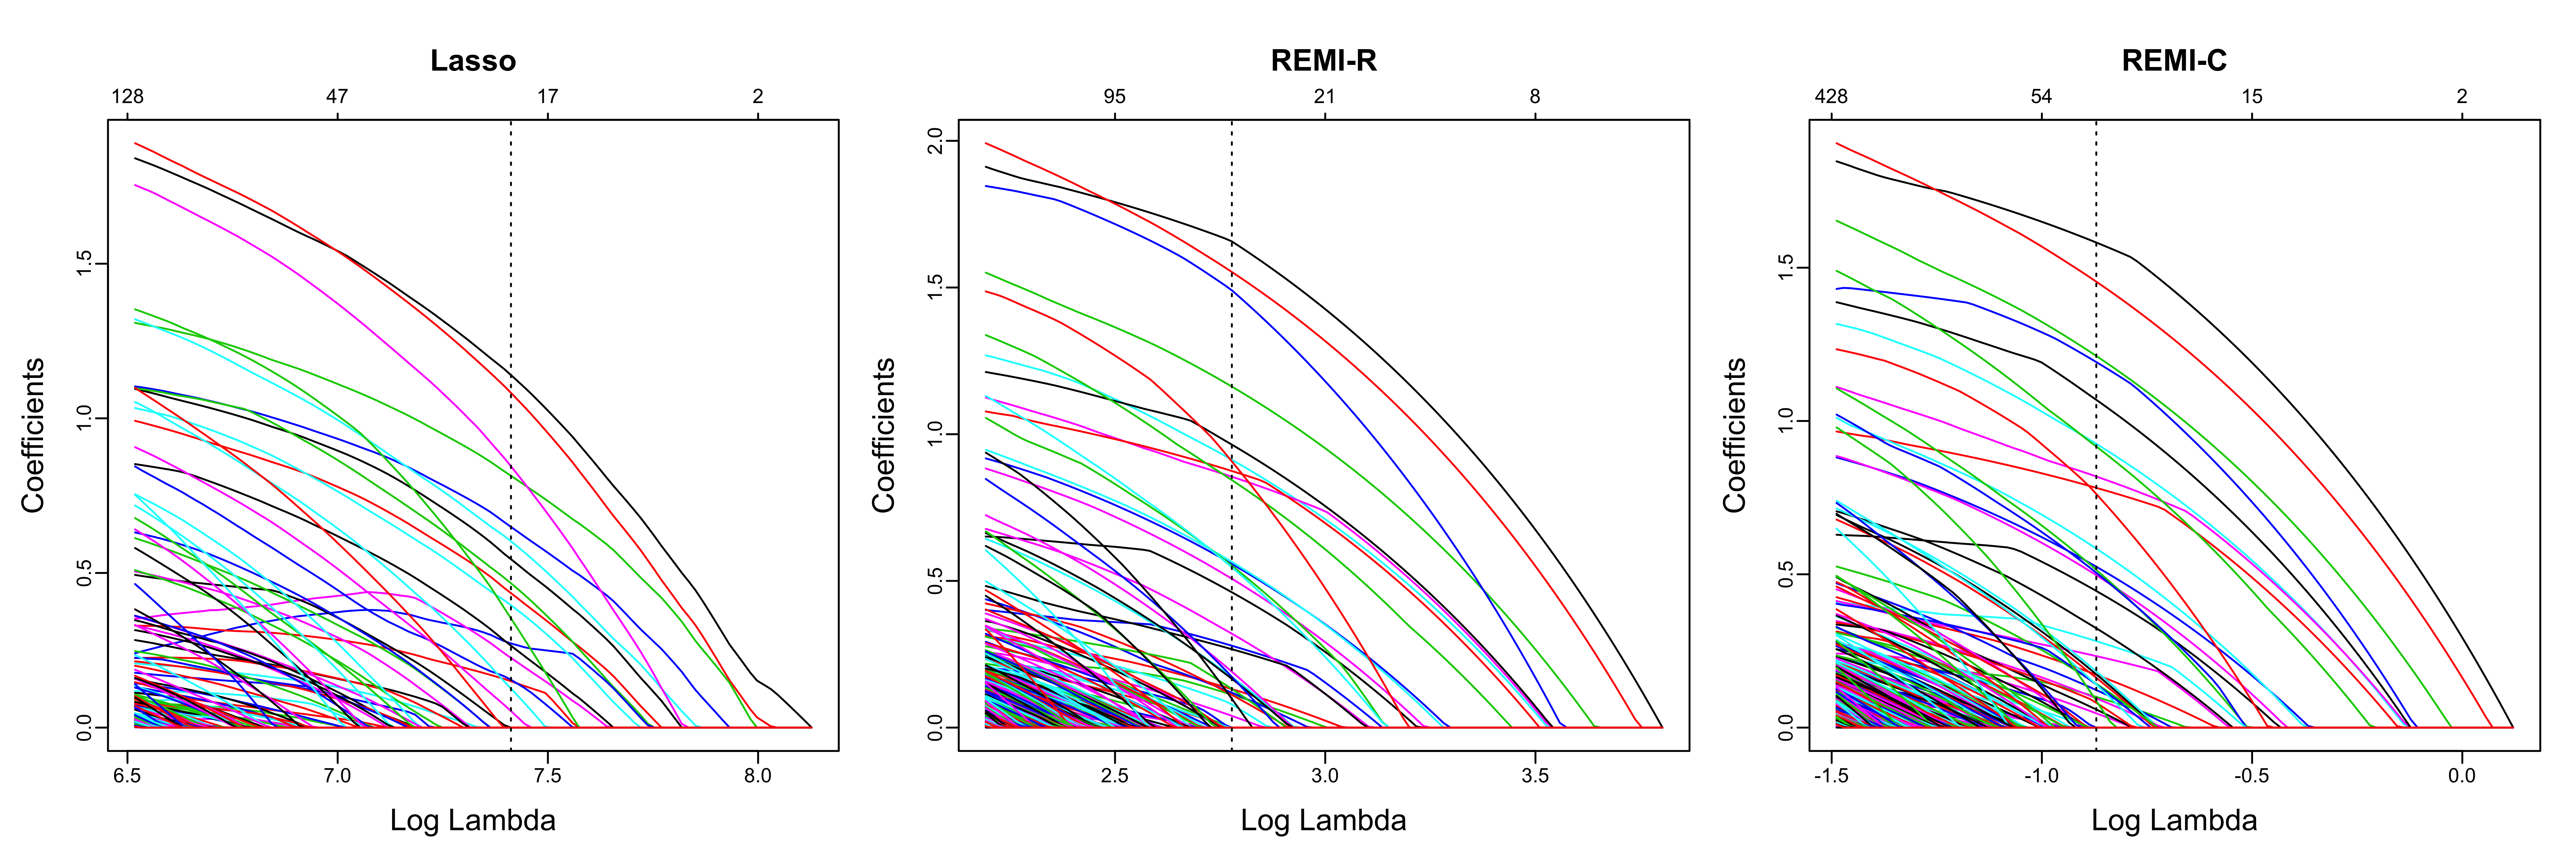
\includegraphics[width=0.8\textwidth]{path_demo.png}

	\caption{Solution paths of Lasso, REMI-R, and REMI-C for a simulated data set.}
	\label{fig}
\end{figure}

\begin{thebibliography}{99}
\bibitem{REMI} Jian Huang, Yuling Jiao, Jin Liu, Can Yang. REMI: Regression with marginal information with applications in genome-wide association studies. 2018. Under review.

\end{thebibliography}

\end{document}
